\chapter{Estrategia}
\section{Introduccion}
Además de los elementos de motivación descritos en el \autoref{chap:Motivacional}, el lenguaje también incluye una serie de elementos de estrategia, en particular la capacidad, los recursos y el curso de acción, como se muestra en la figura 5.1. Estos se definen como especializaciones de los elementos genéricos de comportamiento y estructura y se definen con más detalle en las siguientes secciones. \\

Para describir los aspectos estratégicos de la empresa se han definido los puntos de vista que se exponen a continuación. Cada uno de estos puntos de vista presenta una perspectiva diferente de la modelización de la dirección estratégica de alto nivel y de la composición de la empresa y permite a un modelador centrarse en determinados aspectos. Por lo tanto, cada punto de vista considera sólo una selección de los elementos y relaciones que se han descrito en las sección 3.3. Se distinguen los siguientes puntos de vista:

\begin{itemize}
	\item El punto de vista del mapa de capacidades proporciona una visión general de las capacidades de la empresa.
	\item El punto de vista de la realización de resultados describe la forma en que los resultados de alto nivel y orientados a los negocios se producen gracias a las capacidades y recursos de la empresa.
	\item El punto de vista del mapa de recursos proporciona una visión general estructurada de los recursos de la empresa.
\end{itemize}

\newpage

\section{Metamodelo}
\begin{figure}[h!]
	\centering
	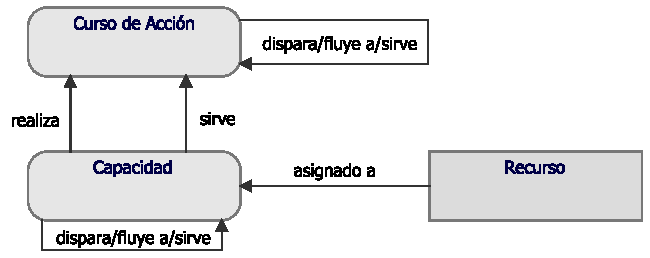
\includegraphics[width=0.9\linewidth]{imgs/meta/Estrategia}
	\caption{Metamodelo Motivacional}
\end{figure}

La figura 5.1 ofrece una visión general de los elementos de la estrategia y sus relaciones. Un recurso representa un activo que pertenece o está controlado por un individuo u organización.
Los recursos son un concepto central en el campo de la gestión estratégica, la economía, la informática, la gestión de carteras y más. A menudo se consideran, junto con las capacidades, como fuentes de ventaja competitiva para las organizaciones. Una capacidad representa una habilidad que posee un elemento de estructura activa, como una organización, una persona o un sistema.
En el ámbito de los negocios, el pensamiento y la planificación estratégicos proporcionan estrategias y objetivos de alto nivel que a menudo no se pueden aplicar directamente en la arquitectura de una organización. Un curso de acción es un enfoque o plan para configurar algunas capacidades y recursos de la empresa, emprendido para lograr un objetivo. Un curso de acción representa lo que una empresa ha decidido hacer. Los cursos de acción pueden ser categorizados como estrategias y tácticas. No es posible hacer una distinción estricta entre ambos, pero las estrategias tienden a ser a largo plazo y de alcance bastante amplio, mientras que las tácticas tienden a ser a corto plazo y de alcance más limitado.

\newpage
\chapter{Estrategia}
\section{Introduccion}
Además de los elementos de motivación descritos en el \ref{chap:Motivacional}, el lenguaje también incluye una serie de elementos de estrategia, en particular la capacidad, los recursos y el curso de acción, como se muestra en la figura 4. Estos se definen como especializaciones de los elementos genéricos de comportamiento y estructura y se definen con más detalle en el capítulo 7.

\newpage

\section{Metamodelo}
\begin{figure}[h!]
	\centering
	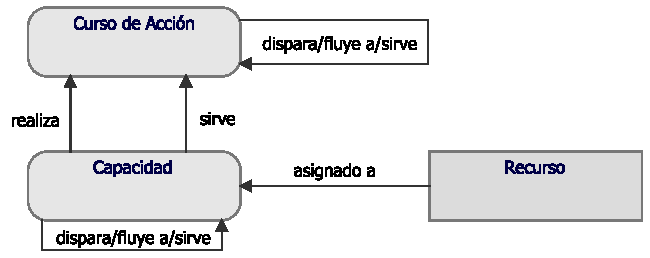
\includegraphics[width=0.9\linewidth]{imgs/meta/Estrategia}
	\caption{Metamodelo Motivacional}
\end{figure}

descripcion....

\newpage
\chapter{Estrategia}
\section{Introduccion}
Además de los elementos de motivación descritos en el \ref{chap:Motivacional}, el lenguaje también incluye una serie de elementos de estrategia, en particular la capacidad, los recursos y el curso de acción, como se muestra en la figura 4. Estos se definen como especializaciones de los elementos genéricos de comportamiento y estructura y se definen con más detalle en el capítulo 7.

\newpage

\section{Metamodelo}
\begin{figure}[h!]
	\centering
	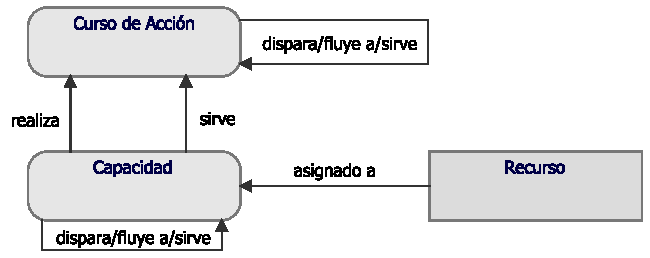
\includegraphics[width=0.9\linewidth]{imgs/meta/Estrategia}
	\caption{Metamodelo Motivacional}
\end{figure}

descripcion....

\newpage
\chapter{Estrategia}
\section{Introduccion}
Además de los elementos de motivación descritos en el \ref{chap:Motivacional}, el lenguaje también incluye una serie de elementos de estrategia, en particular la capacidad, los recursos y el curso de acción, como se muestra en la figura 4. Estos se definen como especializaciones de los elementos genéricos de comportamiento y estructura y se definen con más detalle en el capítulo 7.

\newpage

\section{Metamodelo}
\begin{figure}[h!]
	\centering
	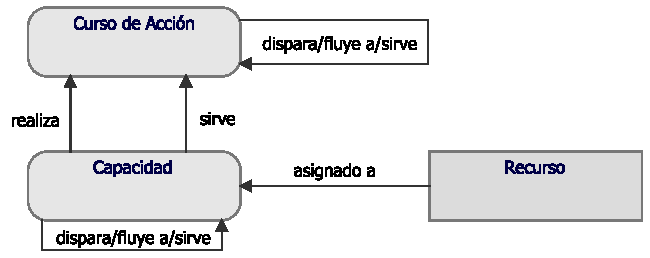
\includegraphics[width=0.9\linewidth]{imgs/meta/Estrategia}
	\caption{Metamodelo Motivacional}
\end{figure}

descripcion....

\newpage
\include{arquitectura/estrategia/estrategia}

\newpage
\include{arquitectura/estrategia/capacidad}


\newpage
\include{arquitectura/estrategia/resultado}

\newpage
\include{arquitectura/estrategia/recurso}



\newpage
\section{Punto de Vista de Mapa de Capacidad}

El punto de vista del mapa de capacidades permite al arquitecto de la empresa crear una visión general estructurada de las capacidades de la empresa. Un mapa de capacidad típicamente muestra dos o tres niveles de capacidades en toda la empresa. Puede, por ejemplo, utilizarse como mapa de calor para identificar áreas de inversión. En algunos casos, un mapa de capacidades también puede mostrar los resultados específicos que ofrecen esas capacidades.

\subsection{Modelo de Mapa de Capacidad}
\begin{figure}[h!]
	\centering
	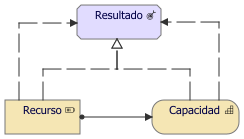
\includegraphics[width=.5\linewidth]{imgs/caso/MapaCapacidad}
	\caption{Modelo Mapa de Capacidad}
\end{figure}

En sínstesis, un recurso es un activo que es propiedad o está controlado por un individuo u organización. Por otra parte, una capacidad es una habilidad que posee un elemento de estructura activa, como una organización, una persona o un sistema. Y, finalmente, un curso de acción es un enfoque o plan para configurar algunas capacidades y recursos de la empresa, dispustos para la consecusión de un objetivo. \\

Aumentar el beneficio es un objetivo que puede descomponerse en varios otros objetivos: Disminuir los costos y aumentar los ingresos. El primero está relacionado con la estrategia de Operación Excelencia de la empresa, modelada como un curso de acción. Estos resultan en dos resultados: Disminución de los costos y pérdida de clientes, que influyen en los objetivos de manera positiva y negativa. Esto muestra una importante diferencia entre los objetivos y los resultados: no todos los resultados conducen a los resultados previstos.
Los cursos de acción se realizan por una serie de capacidades: Gestión y operaciones de TI y gestión de productos, y los recursos apropiados Recursos humanos y recursos de TI se asignan a las primeras.

\newpage

\subsection{Caso de Mapa de Capacidad}

\subsubsection{Resutlado 1: Mejores Investigadores e Investigaciones}

\begin{figure}[h!]
	\centering
	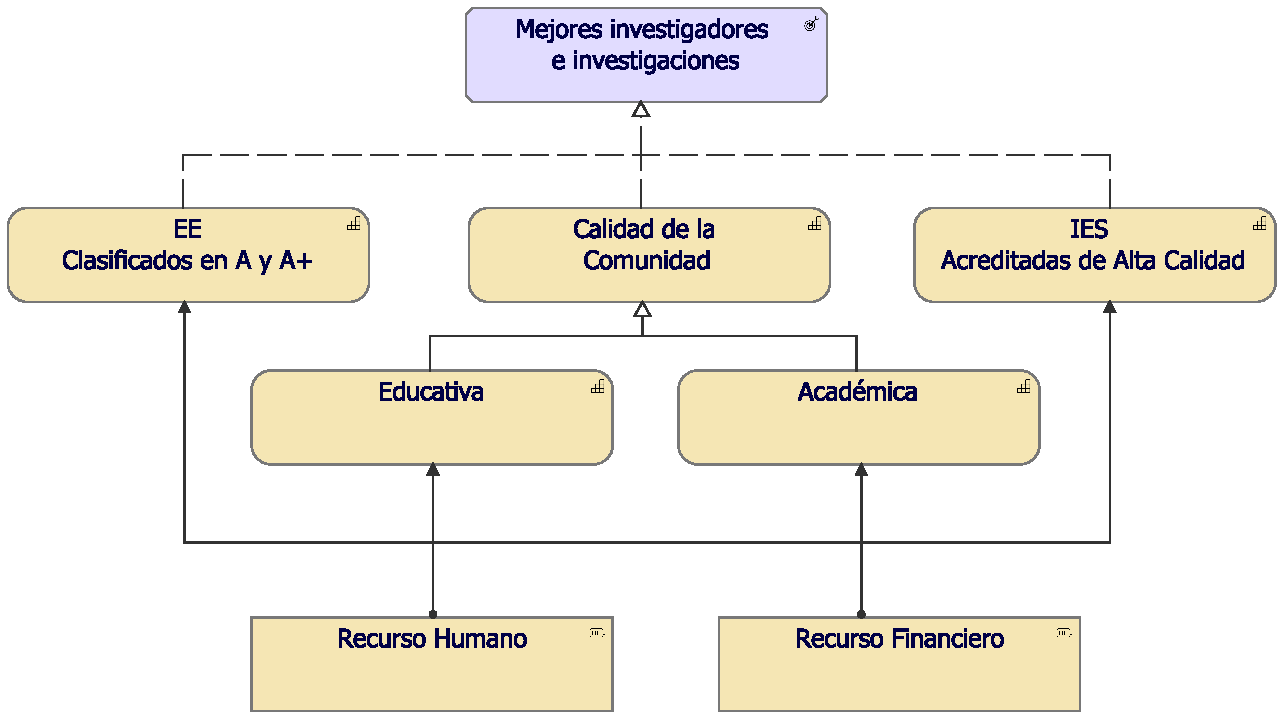
\includegraphics[width=1\linewidth]{imgs/modelo/estrategia/capacidad/1.pdf}
	\caption{Caso Mapa de Capacidad}
\end{figure}

Para dar alcance al resultado de obtener mejores investigadores y mejores investigaciones, el MEN como estructura activa se basa en las habilidades inmersas tanto en los Establecimientos Educativos de calificación A y A+ \footnote{\url{https://www.icfes.gov.co/documents/20143/193495/Clasificacion+de+establecimientos+y+sedes+Saber+11.pdf/2f177381-3c38-6b20-f5da-272dba42b412}}, los cuales representan la mayoría de los planteles registrados, así como las habilidades al interior de sus Instituciones de Educación Superior acreditadas de alta calidad. \\

No obstante, estas habilidades se encuentran arraigadas a la capacidad provista por la calidad de la comunidad, educativa y académica respectivamente. A saber, el activo más importante del MEN, el recurso humano; y que, junto al recurso financiero, conforman el punto de partida para el curso de acción de la organización.

\clearpage
\subsubsection{Resutlado 2: Generación de Estudiantes de Alta Calidad}

\begin{figure}[h!]
	\centering
	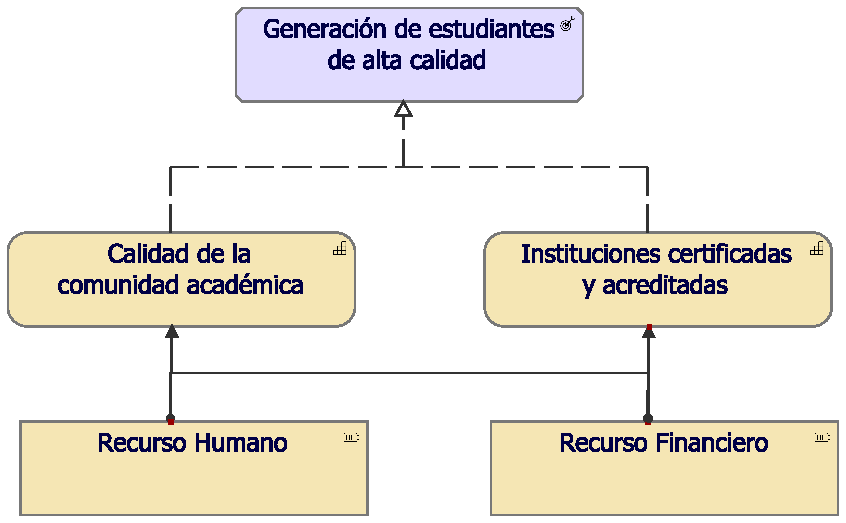
\includegraphics[width=.7\linewidth]{imgs/modelo/estrategia/capacidad/2.pdf}
	\caption{Caso Mapa de Capacidad}
\end{figure}

En en el marco de la \textbf{generación de estudiantes} de alta calidad, el MEN dispone de dos capacidades como lo son la calidad de la comunidad académica e instituciones certificadas y acreditadas que garantizan el desarrollo de procesos con altos estándares de calidad. Las cuales, junto con los recursos humano y financiero, se encuntran configurados dentro del curso de acción para la consecusión de dicho objetivo.


\newpage
\section{Punto de Vista de Realización de resultado}

El punto de vista de la realización de resultados se utiliza para mostrar cómo las capacidades y los elementos básicos subyacentes producen resultados de más alto nivel orientados al negocio.

\subsection{Modelo de Realización de resultado}
\begin{figure}[h!]
	\centering
	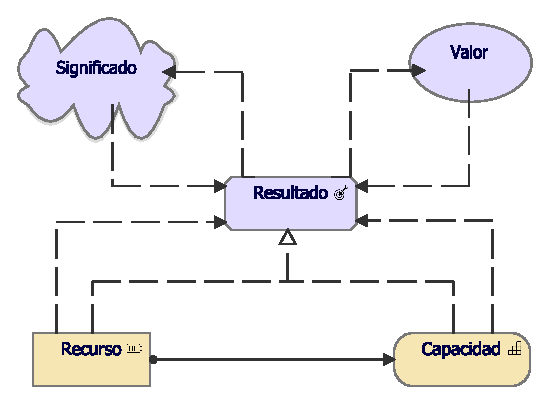
\includegraphics[width=.5\linewidth]{imgs/caso/RealResultado.pdf}
	\caption{Modelo Realización de resultado}
\end{figure}

El punto de vista de la realización de resultados describe cómo las capacidades y los recursos de la empresa producen resultados de alto nivel orientados al negocio.

\newpage

\subsection{Caso de Realización de resultado}

\subsubsection{Resultado 1: Mejores Investigadores e Investigaciones}

\begin{figure}[h!]
	\centering
	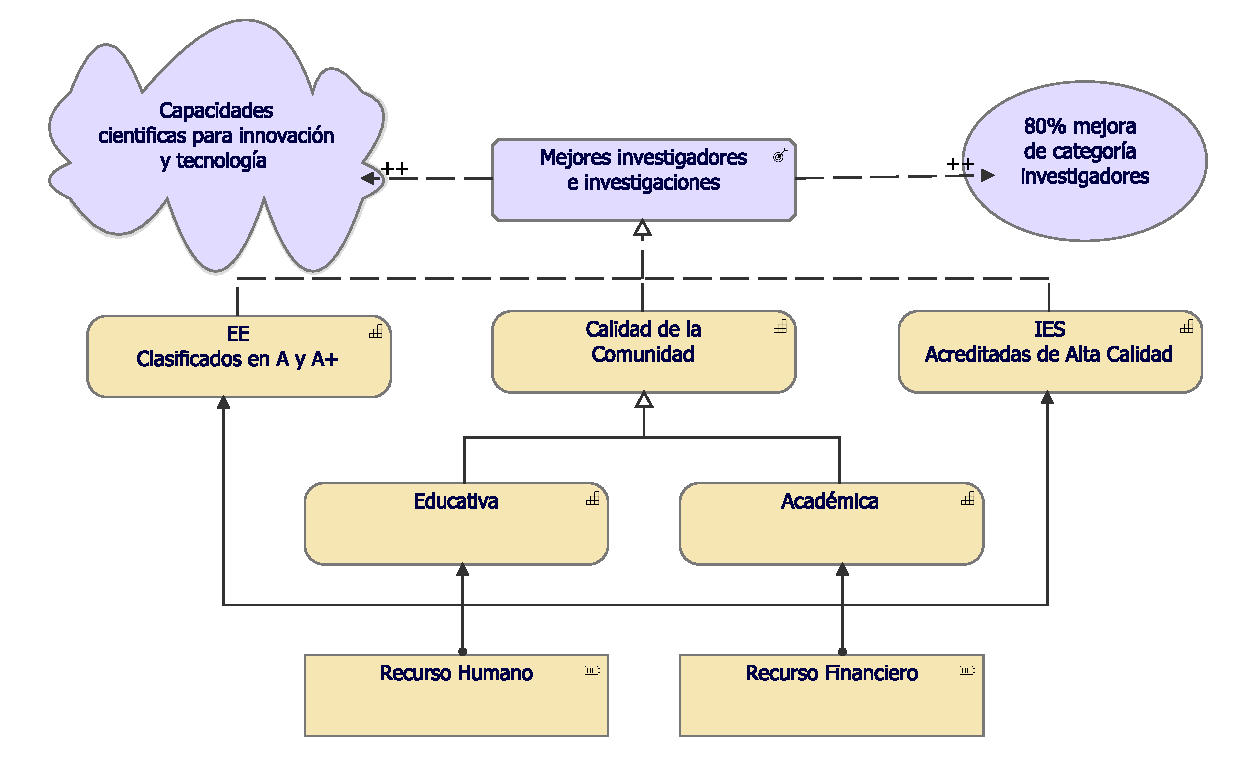
\includegraphics[width=.8\linewidth]{imgs/modelo/estrategia/resultado/resultado_2.pdf}
	\caption{Caso Realización de resultado}
\end{figure}

Para el caso de resultado de \textbf{Mejores Investigadores e Investigaciones} se busca promover nuevas capacidades científicas que fomenten la innovación y la tecnología gracias comunidad de calidad, de las IES acreditadas de alta calidad. Se pretende alcanzar el 80 por ciento en subir de categoría por parte de los investigadores.


\clearpage
\subsubsection{Resultado 2: Generación de Estudiantes de Alta Calidad}

\begin{figure}[h!]
	\centering
	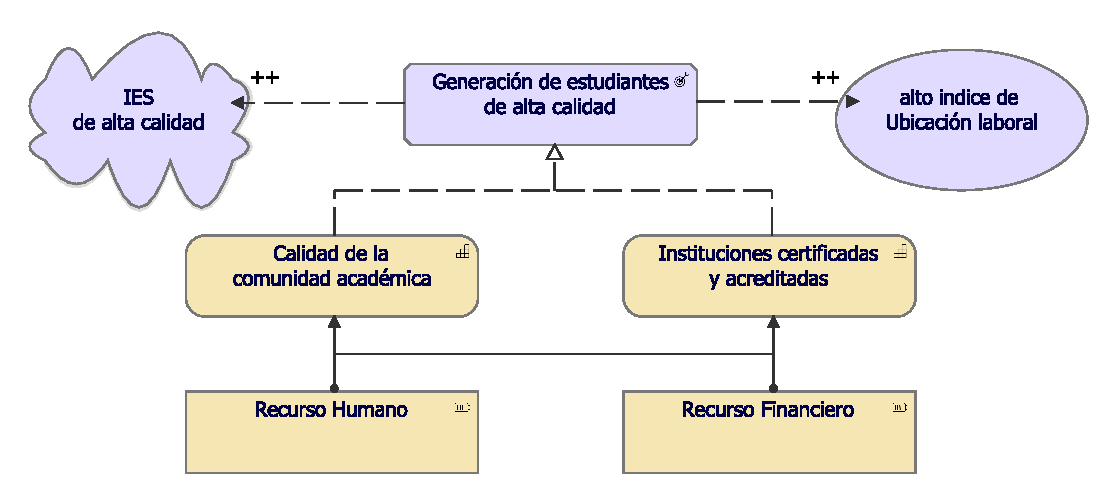
\includegraphics[width=.8\linewidth]{imgs/modelo/estrategia/resultado/resultado.pdf}
	\caption{Caso Realización de resultado}
\end{figure}

El resultado de \textbf{generación de estudiantes de alta calidad} proporciona un significado de grandes expectativas para el MEN, puesto que este resultado da como garantía Instituciones de Educación Superior(IES) de alta calidad promoviendo la capacidad de calidad en la comunidad académica ademas de instituciones certificadas y acreditadas.

\newpage
\section{Punto de Vista de Mapa de Recurso}

El punto de vista del mapa de recursos permite al arquitecto comercial crear una descripción general estructurada de los recursos de la empresa. Un mapa de recursos generalmente muestra dos o tres niveles de recursos en toda la empresa. Puede, por ejemplo, utilizarse como mapa de calor para identificar áreas de inversión. En algunos casos, un mapa de recursos también puede mostrar relaciones entre los recursos y las capacidades a las que están asignados.

\subsection{Modelo de Mapa de Recurso}
\begin{figure}[h!]
	\centering
	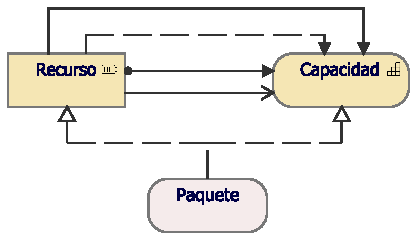
\includegraphics[width=.5\linewidth]{imgs/caso/MapaRecurso.pdf}
	\caption{Modelo Mapa de Recurso}
\end{figure}

El punto de vista del mapa de recursos proporciona una descripción estructurada de los recursos de la empresa.

\newpage

\subsection{Caso de Mapa de Recurso}

\subsubsection{Resultado 1: Mejores Investigadores e Investigaciones}

\begin{figure}[h!]
	\centering
	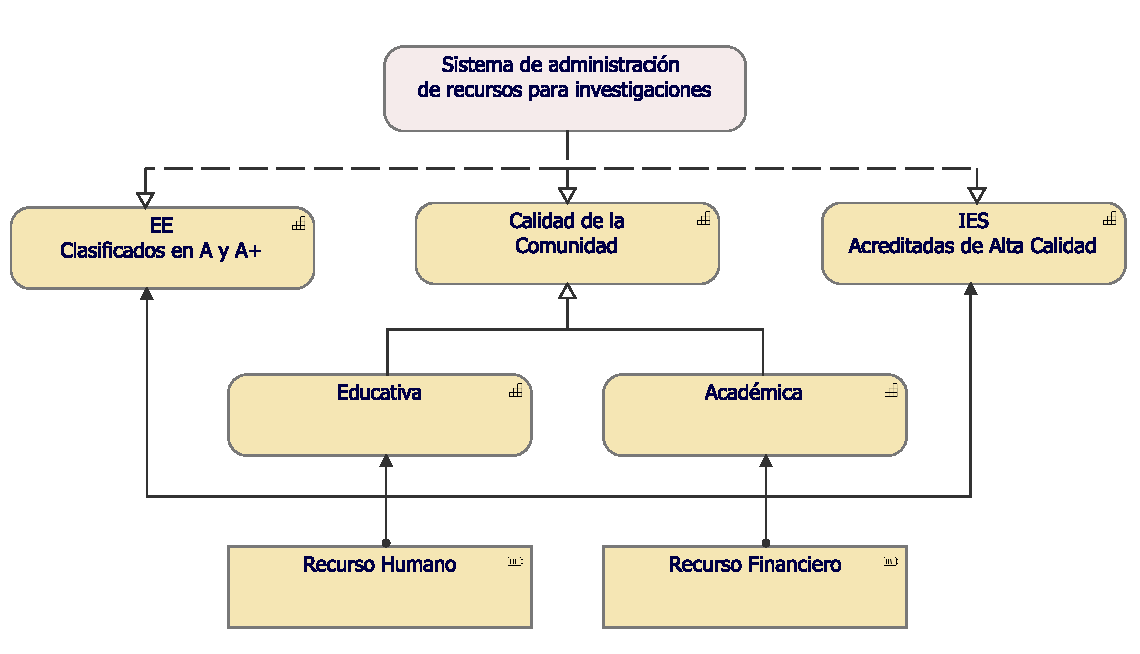
\includegraphics[width=1\linewidth]{imgs/modelo/estrategia/mapa/mapa_recurso.pdf}
	\caption{Caso Mapa de Recurso}
\end{figure}

Para dar alcance a las capacidades de calidad de la comunidad, IES Acreditadas de Alta Calidad y EE Clasificados en A y A+ basadas en habilidades dadas por el resultado de Mejores Investigadores e Investigaciones, se pretende construir un sistema que administre de manera optima los recursos para realizar nuevas investigaciones dando lugar a un crecimiento exponencial de nuevos investigadores.

\clearpage
\subsubsection{Resultado 2: Generación de Estudiantes de Alta Calidad}

\begin{figure}[h!]
	\centering
	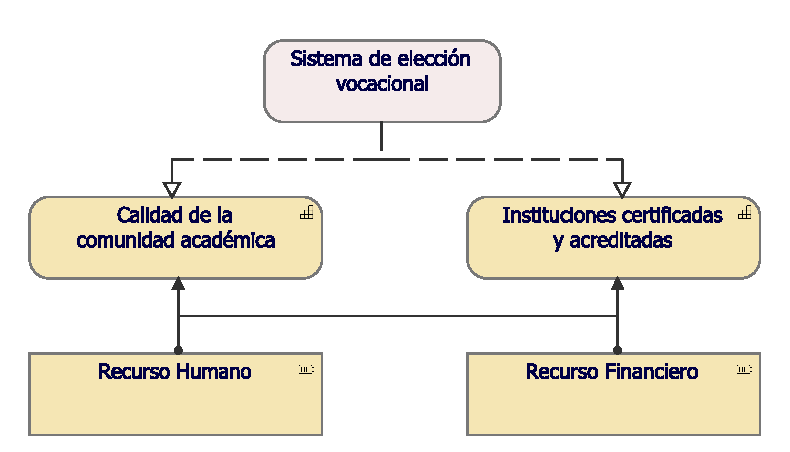
\includegraphics[width=.8\linewidth]{imgs/modelo/estrategia/mapa/mapa_recurso_2.pdf}
	\caption{Caso Mapa de Recurso}
\end{figure}

Para garantizar la generación de estudiantes de calidad es necesario implantar nuevos sistemas que ayudan a elegir de mejor manera la vocación que tendrán en el futuro los estudiantes. Buscando así que el estudiante se acerque a las diferentes carreras o áreas del conocimiento sin sentir presión por parte de ningún ente, que aquella vocación escogida por el estudiante sea totalmente de su agrado y gusto; formando estudiantes que lleven la educación de calidad no por obligación sino por interés propio.



\newpage
\section{Punto de Vista de Mapa de Capacidad}

El punto de vista del mapa de capacidades permite al arquitecto de la empresa crear una visión general estructurada de las capacidades de la empresa. Un mapa de capacidad típicamente muestra dos o tres niveles de capacidades en toda la empresa. Puede, por ejemplo, utilizarse como mapa de calor para identificar áreas de inversión. En algunos casos, un mapa de capacidades también puede mostrar los resultados específicos que ofrecen esas capacidades.

\subsection{Modelo de Mapa de Capacidad}
\begin{figure}[h!]
	\centering
	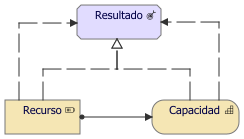
\includegraphics[width=.5\linewidth]{imgs/caso/MapaCapacidad}
	\caption{Modelo Mapa de Capacidad}
\end{figure}

En sínstesis, un recurso es un activo que es propiedad o está controlado por un individuo u organización. Por otra parte, una capacidad es una habilidad que posee un elemento de estructura activa, como una organización, una persona o un sistema. Y, finalmente, un curso de acción es un enfoque o plan para configurar algunas capacidades y recursos de la empresa, dispustos para la consecusión de un objetivo. \\

Aumentar el beneficio es un objetivo que puede descomponerse en varios otros objetivos: Disminuir los costos y aumentar los ingresos. El primero está relacionado con la estrategia de Operación Excelencia de la empresa, modelada como un curso de acción. Estos resultan en dos resultados: Disminución de los costos y pérdida de clientes, que influyen en los objetivos de manera positiva y negativa. Esto muestra una importante diferencia entre los objetivos y los resultados: no todos los resultados conducen a los resultados previstos.
Los cursos de acción se realizan por una serie de capacidades: Gestión y operaciones de TI y gestión de productos, y los recursos apropiados Recursos humanos y recursos de TI se asignan a las primeras.

\newpage

\subsection{Caso de Mapa de Capacidad}

\subsubsection{Resutlado 1: Mejores Investigadores e Investigaciones}

\begin{figure}[h!]
	\centering
	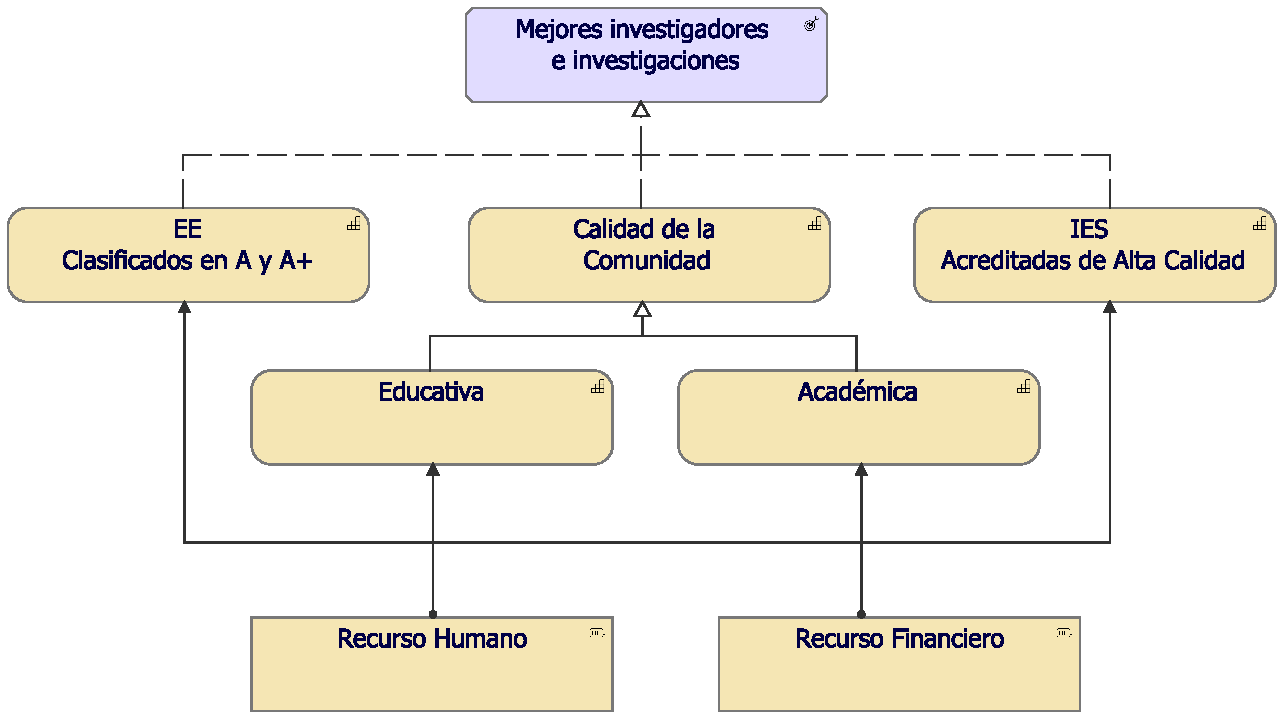
\includegraphics[width=1\linewidth]{imgs/modelo/estrategia/capacidad/1.pdf}
	\caption{Caso Mapa de Capacidad}
\end{figure}

Para dar alcance al resultado de obtener mejores investigadores y mejores investigaciones, el MEN como estructura activa se basa en las habilidades inmersas tanto en los Establecimientos Educativos de calificación A y A+ \footnote{\url{https://www.icfes.gov.co/documents/20143/193495/Clasificacion+de+establecimientos+y+sedes+Saber+11.pdf/2f177381-3c38-6b20-f5da-272dba42b412}}, los cuales representan la mayoría de los planteles registrados, así como las habilidades al interior de sus Instituciones de Educación Superior acreditadas de alta calidad. \\

No obstante, estas habilidades se encuentran arraigadas a la capacidad provista por la calidad de la comunidad, educativa y académica respectivamente. A saber, el activo más importante del MEN, el recurso humano; y que, junto al recurso financiero, conforman el punto de partida para el curso de acción de la organización.

\clearpage
\subsubsection{Resutlado 2: Generación de Estudiantes de Alta Calidad}

\begin{figure}[h!]
	\centering
	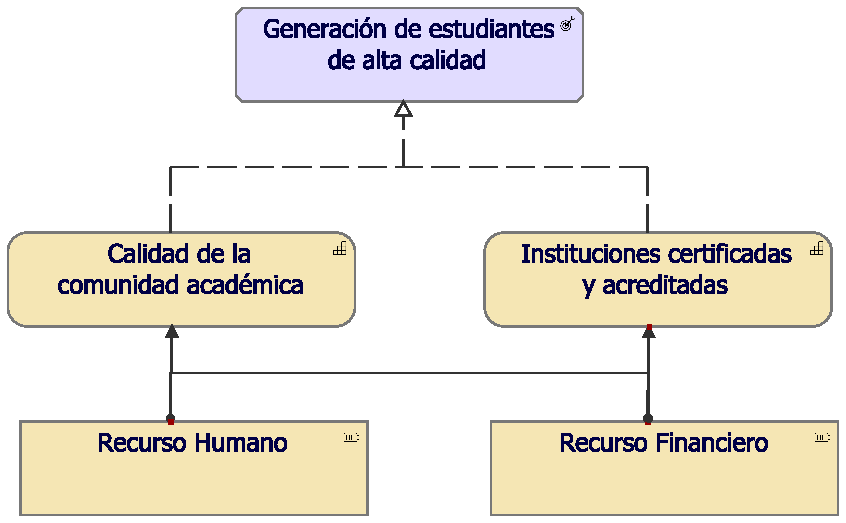
\includegraphics[width=.7\linewidth]{imgs/modelo/estrategia/capacidad/2.pdf}
	\caption{Caso Mapa de Capacidad}
\end{figure}

En en el marco de la \textbf{generación de estudiantes} de alta calidad, el MEN dispone de dos capacidades como lo son la calidad de la comunidad académica e instituciones certificadas y acreditadas que garantizan el desarrollo de procesos con altos estándares de calidad. Las cuales, junto con los recursos humano y financiero, se encuntran configurados dentro del curso de acción para la consecusión de dicho objetivo.


\newpage
\section{Punto de Vista de Realización de resultado}

El punto de vista de la realización de resultados se utiliza para mostrar cómo las capacidades y los elementos básicos subyacentes producen resultados de más alto nivel orientados al negocio.

\subsection{Modelo de Realización de resultado}
\begin{figure}[h!]
	\centering
	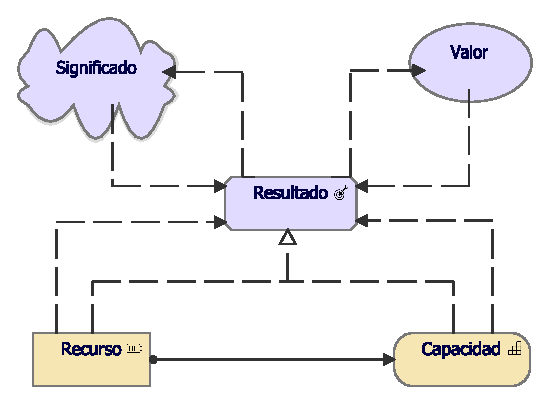
\includegraphics[width=.5\linewidth]{imgs/caso/RealResultado.pdf}
	\caption{Modelo Realización de resultado}
\end{figure}

El punto de vista de la realización de resultados describe cómo las capacidades y los recursos de la empresa producen resultados de alto nivel orientados al negocio.

\newpage

\subsection{Caso de Realización de resultado}

\subsubsection{Resultado 1: Mejores Investigadores e Investigaciones}

\begin{figure}[h!]
	\centering
	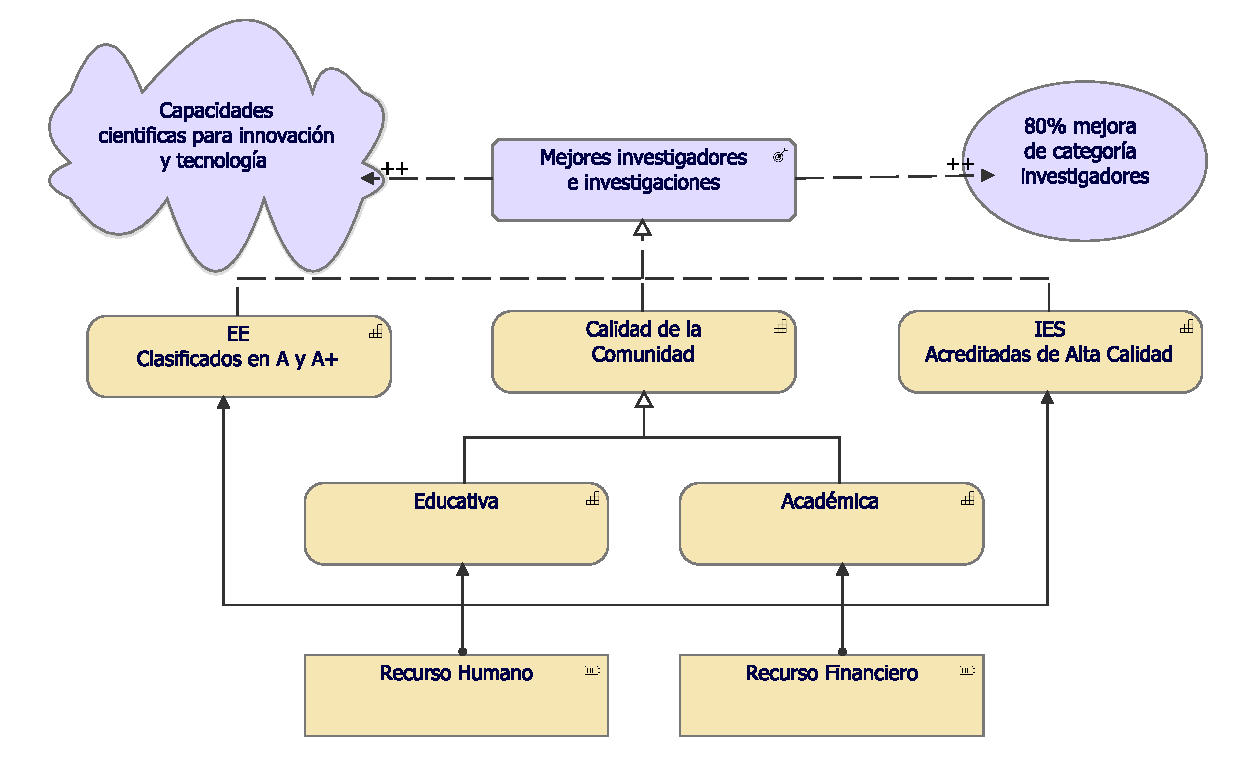
\includegraphics[width=.8\linewidth]{imgs/modelo/estrategia/resultado/resultado_2.pdf}
	\caption{Caso Realización de resultado}
\end{figure}

Para el caso de resultado de \textbf{Mejores Investigadores e Investigaciones} se busca promover nuevas capacidades científicas que fomenten la innovación y la tecnología gracias comunidad de calidad, de las IES acreditadas de alta calidad. Se pretende alcanzar el 80 por ciento en subir de categoría por parte de los investigadores.


\clearpage
\subsubsection{Resultado 2: Generación de Estudiantes de Alta Calidad}

\begin{figure}[h!]
	\centering
	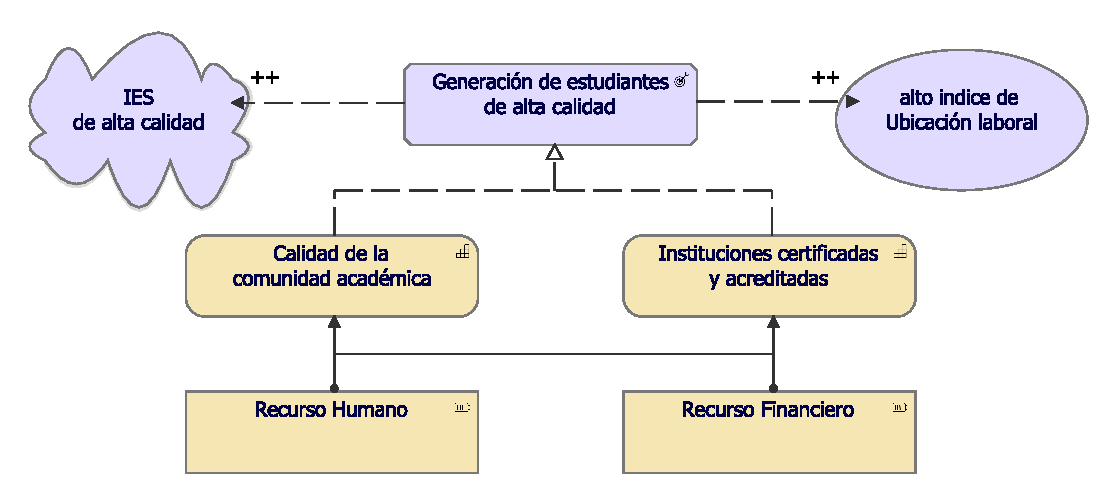
\includegraphics[width=.8\linewidth]{imgs/modelo/estrategia/resultado/resultado.pdf}
	\caption{Caso Realización de resultado}
\end{figure}

El resultado de \textbf{generación de estudiantes de alta calidad} proporciona un significado de grandes expectativas para el MEN, puesto que este resultado da como garantía Instituciones de Educación Superior(IES) de alta calidad promoviendo la capacidad de calidad en la comunidad académica ademas de instituciones certificadas y acreditadas.

\newpage
\section{Punto de Vista de Mapa de Recurso}

El punto de vista del mapa de recursos permite al arquitecto comercial crear una descripción general estructurada de los recursos de la empresa. Un mapa de recursos generalmente muestra dos o tres niveles de recursos en toda la empresa. Puede, por ejemplo, utilizarse como mapa de calor para identificar áreas de inversión. En algunos casos, un mapa de recursos también puede mostrar relaciones entre los recursos y las capacidades a las que están asignados.

\subsection{Modelo de Mapa de Recurso}
\begin{figure}[h!]
	\centering
	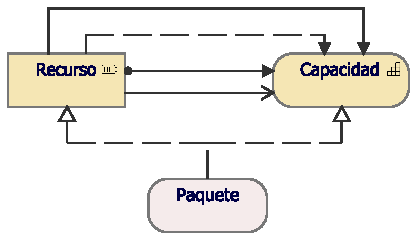
\includegraphics[width=.5\linewidth]{imgs/caso/MapaRecurso.pdf}
	\caption{Modelo Mapa de Recurso}
\end{figure}

El punto de vista del mapa de recursos proporciona una descripción estructurada de los recursos de la empresa.

\newpage

\subsection{Caso de Mapa de Recurso}

\subsubsection{Resultado 1: Mejores Investigadores e Investigaciones}

\begin{figure}[h!]
	\centering
	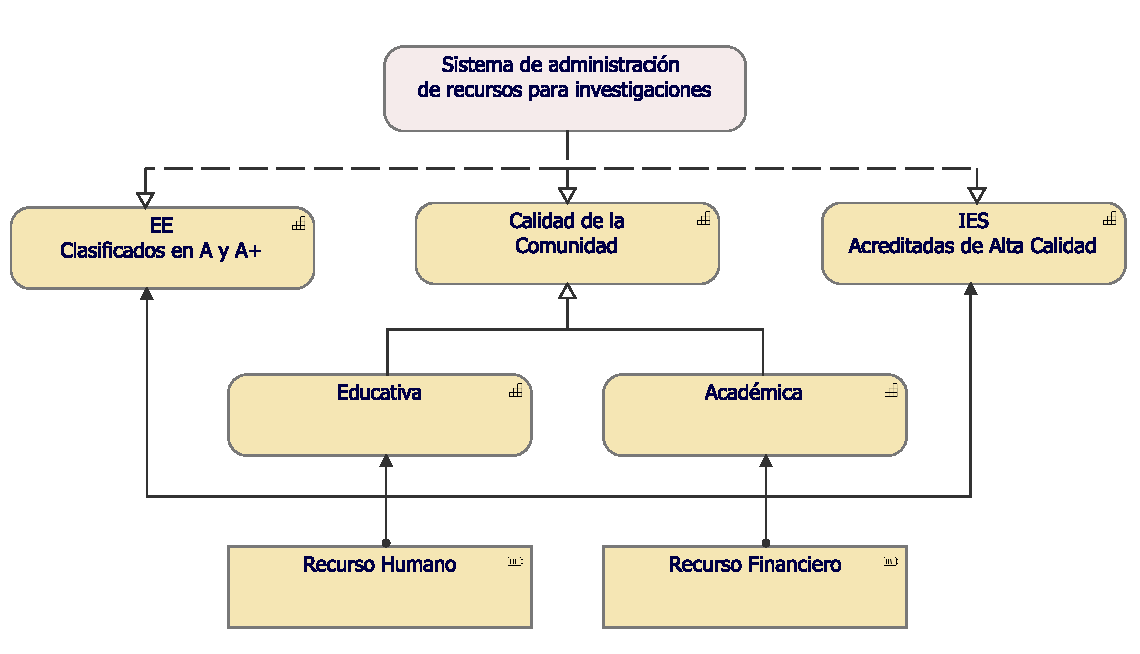
\includegraphics[width=1\linewidth]{imgs/modelo/estrategia/mapa/mapa_recurso.pdf}
	\caption{Caso Mapa de Recurso}
\end{figure}

Para dar alcance a las capacidades de calidad de la comunidad, IES Acreditadas de Alta Calidad y EE Clasificados en A y A+ basadas en habilidades dadas por el resultado de Mejores Investigadores e Investigaciones, se pretende construir un sistema que administre de manera optima los recursos para realizar nuevas investigaciones dando lugar a un crecimiento exponencial de nuevos investigadores.

\clearpage
\subsubsection{Resultado 2: Generación de Estudiantes de Alta Calidad}

\begin{figure}[h!]
	\centering
	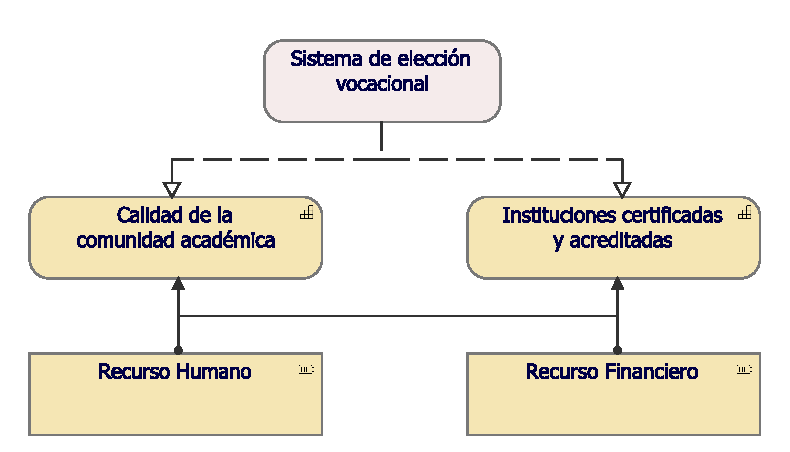
\includegraphics[width=.8\linewidth]{imgs/modelo/estrategia/mapa/mapa_recurso_2.pdf}
	\caption{Caso Mapa de Recurso}
\end{figure}

Para garantizar la generación de estudiantes de calidad es necesario implantar nuevos sistemas que ayudan a elegir de mejor manera la vocación que tendrán en el futuro los estudiantes. Buscando así que el estudiante se acerque a las diferentes carreras o áreas del conocimiento sin sentir presión por parte de ningún ente, que aquella vocación escogida por el estudiante sea totalmente de su agrado y gusto; formando estudiantes que lleven la educación de calidad no por obligación sino por interés propio.



\newpage
\section{Punto de Vista de Mapa de Capacidad}

El punto de vista del mapa de capacidades permite al arquitecto de la empresa crear una visión general estructurada de las capacidades de la empresa. Un mapa de capacidad típicamente muestra dos o tres niveles de capacidades en toda la empresa. Puede, por ejemplo, utilizarse como mapa de calor para identificar áreas de inversión. En algunos casos, un mapa de capacidades también puede mostrar los resultados específicos que ofrecen esas capacidades.

\subsection{Modelo de Mapa de Capacidad}
\begin{figure}[h!]
	\centering
	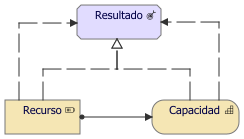
\includegraphics[width=.5\linewidth]{imgs/caso/MapaCapacidad}
	\caption{Modelo Mapa de Capacidad}
\end{figure}

En sínstesis, un recurso es un activo que es propiedad o está controlado por un individuo u organización. Por otra parte, una capacidad es una habilidad que posee un elemento de estructura activa, como una organización, una persona o un sistema. Y, finalmente, un curso de acción es un enfoque o plan para configurar algunas capacidades y recursos de la empresa, dispustos para la consecusión de un objetivo. \\

Aumentar el beneficio es un objetivo que puede descomponerse en varios otros objetivos: Disminuir los costos y aumentar los ingresos. El primero está relacionado con la estrategia de Operación Excelencia de la empresa, modelada como un curso de acción. Estos resultan en dos resultados: Disminución de los costos y pérdida de clientes, que influyen en los objetivos de manera positiva y negativa. Esto muestra una importante diferencia entre los objetivos y los resultados: no todos los resultados conducen a los resultados previstos.
Los cursos de acción se realizan por una serie de capacidades: Gestión y operaciones de TI y gestión de productos, y los recursos apropiados Recursos humanos y recursos de TI se asignan a las primeras.

\newpage

\subsection{Caso de Mapa de Capacidad}

\subsubsection{Resutlado 1: Mejores Investigadores e Investigaciones}

\begin{figure}[h!]
	\centering
	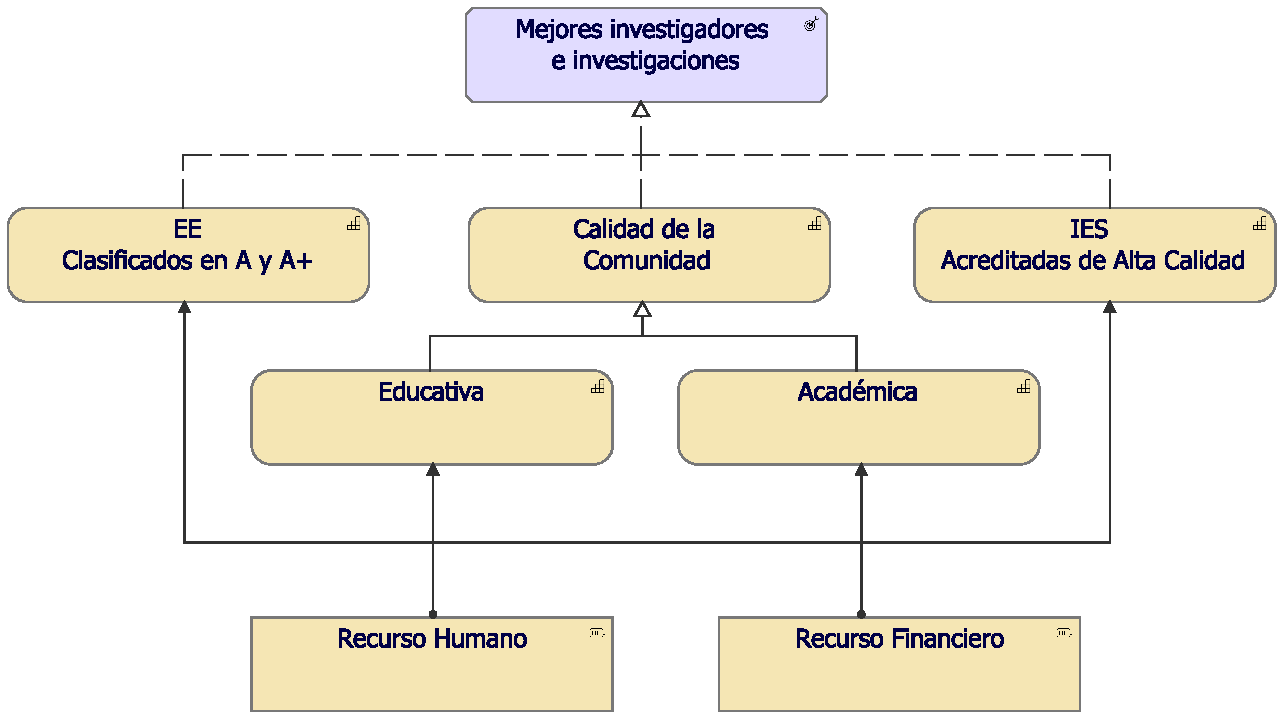
\includegraphics[width=1\linewidth]{imgs/modelo/estrategia/capacidad/1.pdf}
	\caption{Caso Mapa de Capacidad}
\end{figure}

Para dar alcance al resultado de obtener mejores investigadores y mejores investigaciones, el MEN como estructura activa se basa en las habilidades inmersas tanto en los Establecimientos Educativos de calificación A y A+ \footnote{\url{https://www.icfes.gov.co/documents/20143/193495/Clasificacion+de+establecimientos+y+sedes+Saber+11.pdf/2f177381-3c38-6b20-f5da-272dba42b412}}, los cuales representan la mayoría de los planteles registrados, así como las habilidades al interior de sus Instituciones de Educación Superior acreditadas de alta calidad. \\

No obstante, estas habilidades se encuentran arraigadas a la capacidad provista por la calidad de la comunidad, educativa y académica respectivamente. A saber, el activo más importante del MEN, el recurso humano; y que, junto al recurso financiero, conforman el punto de partida para el curso de acción de la organización.

\clearpage
\subsubsection{Resutlado 2: Generación de Estudiantes de Alta Calidad}

\begin{figure}[h!]
	\centering
	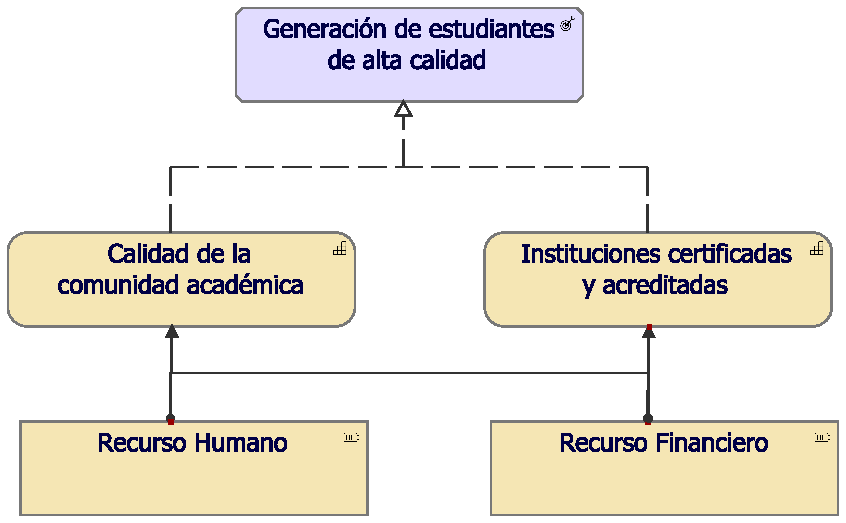
\includegraphics[width=.7\linewidth]{imgs/modelo/estrategia/capacidad/2.pdf}
	\caption{Caso Mapa de Capacidad}
\end{figure}

En en el marco de la \textbf{generación de estudiantes} de alta calidad, el MEN dispone de dos capacidades como lo son la calidad de la comunidad académica e instituciones certificadas y acreditadas que garantizan el desarrollo de procesos con altos estándares de calidad. Las cuales, junto con los recursos humano y financiero, se encuntran configurados dentro del curso de acción para la consecusión de dicho objetivo.


\newpage
\section{Punto de Vista de Realización de resultado}

El punto de vista de la realización de resultados se utiliza para mostrar cómo las capacidades y los elementos básicos subyacentes producen resultados de más alto nivel orientados al negocio.

\subsection{Modelo de Realización de resultado}
\begin{figure}[h!]
	\centering
	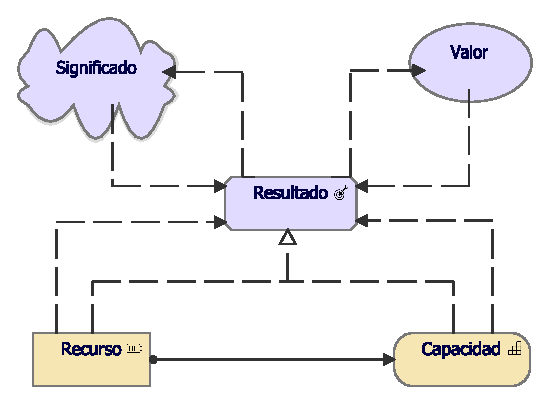
\includegraphics[width=.5\linewidth]{imgs/caso/RealResultado.pdf}
	\caption{Modelo Realización de resultado}
\end{figure}

El punto de vista de la realización de resultados describe cómo las capacidades y los recursos de la empresa producen resultados de alto nivel orientados al negocio.

\newpage

\subsection{Caso de Realización de resultado}

\subsubsection{Resultado 1: Mejores Investigadores e Investigaciones}

\begin{figure}[h!]
	\centering
	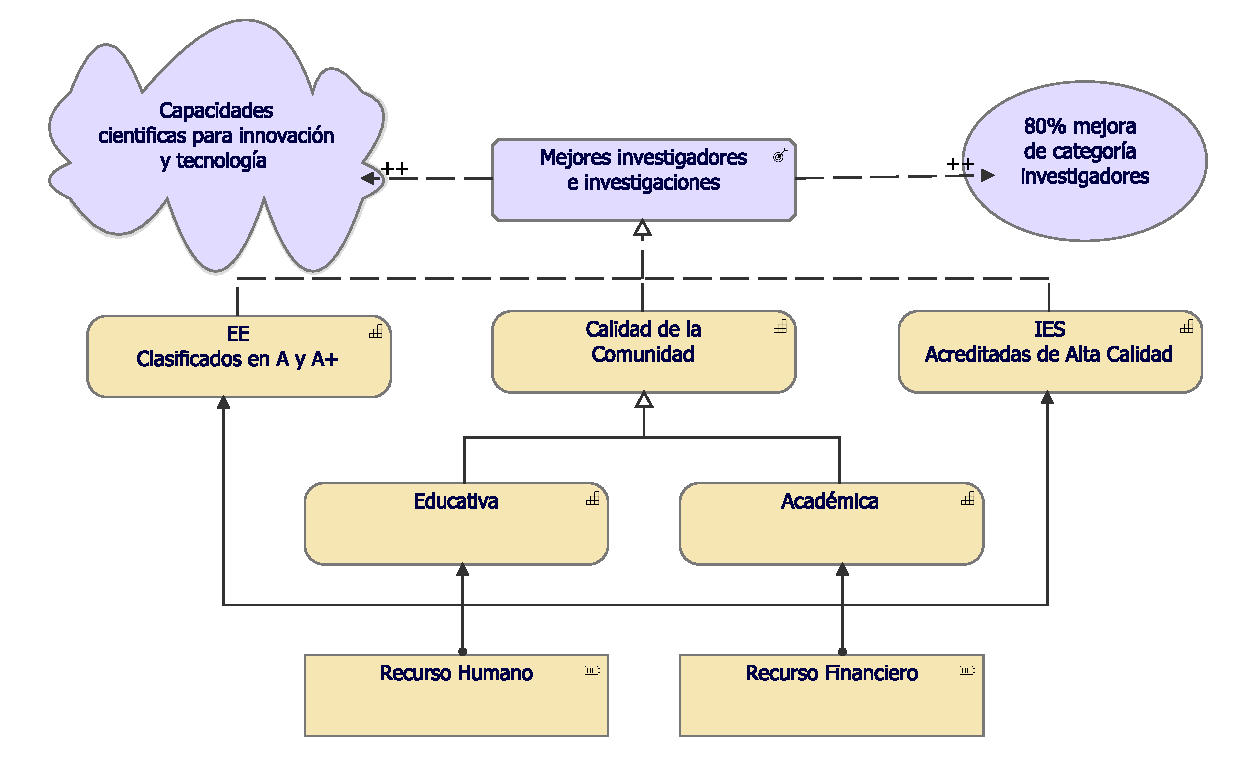
\includegraphics[width=.8\linewidth]{imgs/modelo/estrategia/resultado/resultado_2.pdf}
	\caption{Caso Realización de resultado}
\end{figure}

Para el caso de resultado de \textbf{Mejores Investigadores e Investigaciones} se busca promover nuevas capacidades científicas que fomenten la innovación y la tecnología gracias comunidad de calidad, de las IES acreditadas de alta calidad. Se pretende alcanzar el 80 por ciento en subir de categoría por parte de los investigadores.


\clearpage
\subsubsection{Resultado 2: Generación de Estudiantes de Alta Calidad}

\begin{figure}[h!]
	\centering
	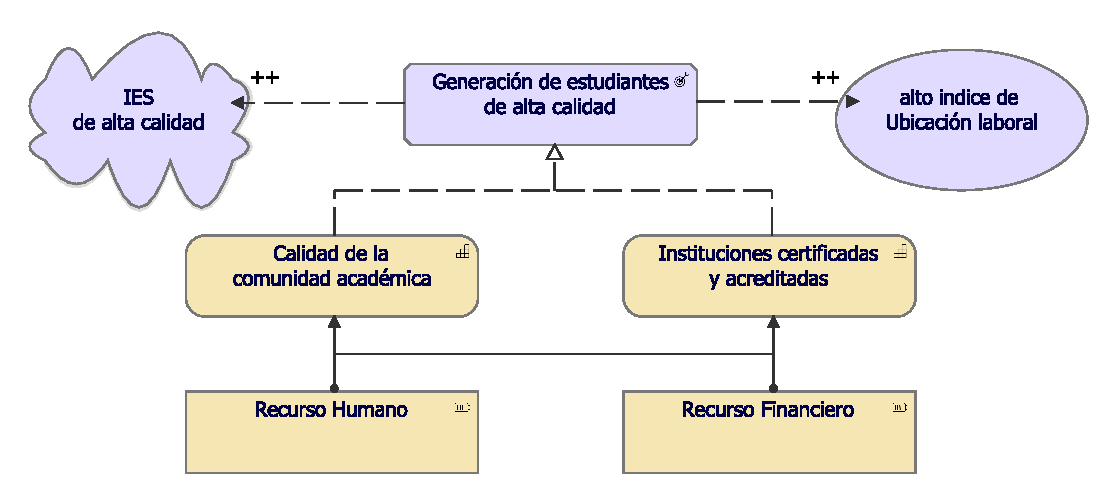
\includegraphics[width=.8\linewidth]{imgs/modelo/estrategia/resultado/resultado.pdf}
	\caption{Caso Realización de resultado}
\end{figure}

El resultado de \textbf{generación de estudiantes de alta calidad} proporciona un significado de grandes expectativas para el MEN, puesto que este resultado da como garantía Instituciones de Educación Superior(IES) de alta calidad promoviendo la capacidad de calidad en la comunidad académica ademas de instituciones certificadas y acreditadas.

\newpage
\section{Punto de Vista de Mapa de Recurso}

El punto de vista del mapa de recursos permite al arquitecto comercial crear una descripción general estructurada de los recursos de la empresa. Un mapa de recursos generalmente muestra dos o tres niveles de recursos en toda la empresa. Puede, por ejemplo, utilizarse como mapa de calor para identificar áreas de inversión. En algunos casos, un mapa de recursos también puede mostrar relaciones entre los recursos y las capacidades a las que están asignados.

\subsection{Modelo de Mapa de Recurso}
\begin{figure}[h!]
	\centering
	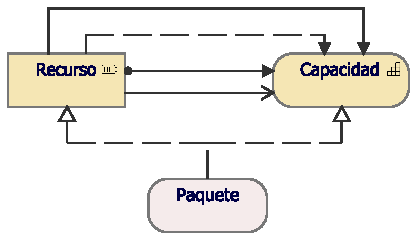
\includegraphics[width=.5\linewidth]{imgs/caso/MapaRecurso.pdf}
	\caption{Modelo Mapa de Recurso}
\end{figure}

El punto de vista del mapa de recursos proporciona una descripción estructurada de los recursos de la empresa.

\newpage

\subsection{Caso de Mapa de Recurso}

\subsubsection{Resultado 1: Mejores Investigadores e Investigaciones}

\begin{figure}[h!]
	\centering
	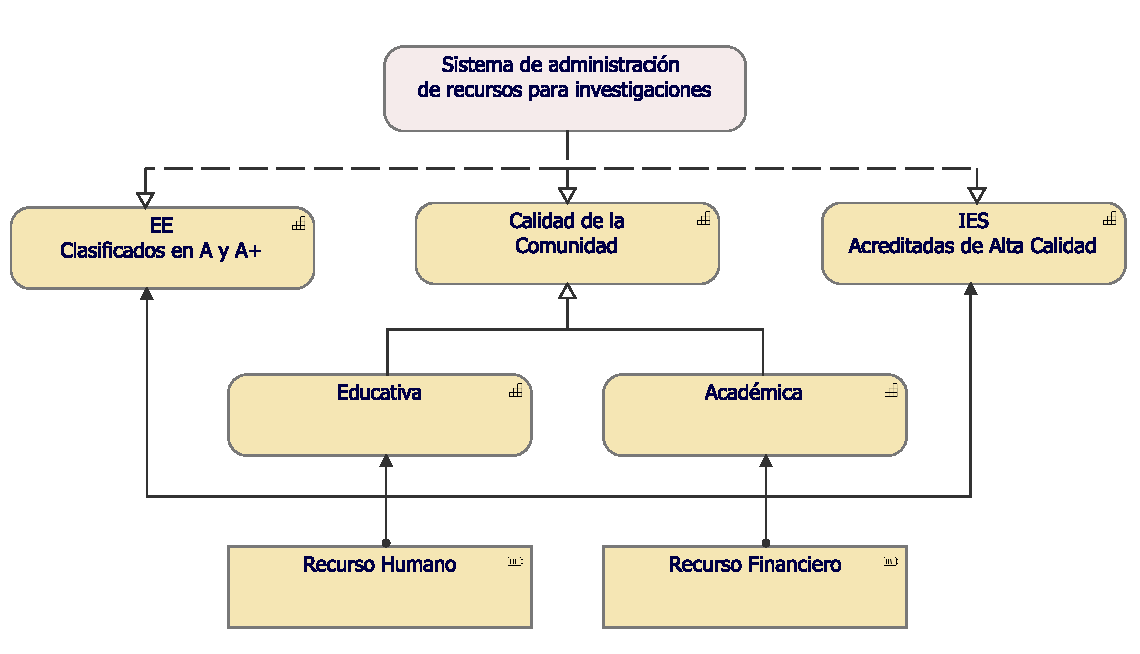
\includegraphics[width=1\linewidth]{imgs/modelo/estrategia/mapa/mapa_recurso.pdf}
	\caption{Caso Mapa de Recurso}
\end{figure}

Para dar alcance a las capacidades de calidad de la comunidad, IES Acreditadas de Alta Calidad y EE Clasificados en A y A+ basadas en habilidades dadas por el resultado de Mejores Investigadores e Investigaciones, se pretende construir un sistema que administre de manera optima los recursos para realizar nuevas investigaciones dando lugar a un crecimiento exponencial de nuevos investigadores.

\clearpage
\subsubsection{Resultado 2: Generación de Estudiantes de Alta Calidad}

\begin{figure}[h!]
	\centering
	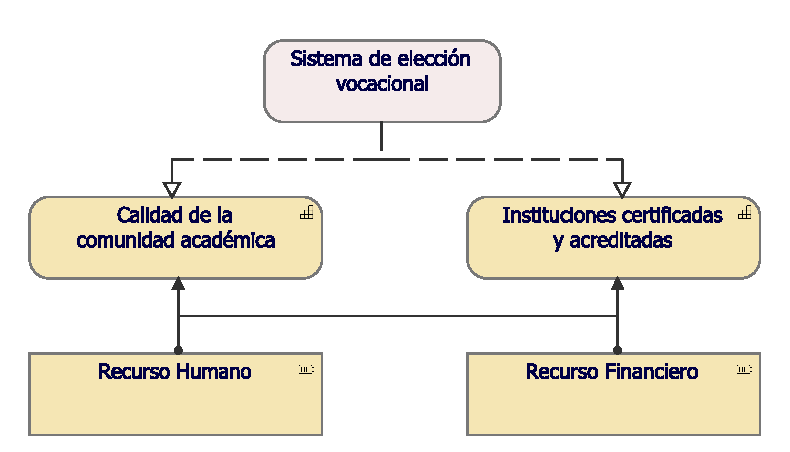
\includegraphics[width=.8\linewidth]{imgs/modelo/estrategia/mapa/mapa_recurso_2.pdf}
	\caption{Caso Mapa de Recurso}
\end{figure}

Para garantizar la generación de estudiantes de calidad es necesario implantar nuevos sistemas que ayudan a elegir de mejor manera la vocación que tendrán en el futuro los estudiantes. Buscando así que el estudiante se acerque a las diferentes carreras o áreas del conocimiento sin sentir presión por parte de ningún ente, que aquella vocación escogida por el estudiante sea totalmente de su agrado y gusto; formando estudiantes que lleven la educación de calidad no por obligación sino por interés propio.

